% Results
\section{Experimental Results}
Three curves were chosen to demonstrate the aspects of the developed 
methods. The first is a family of curves, $Lissajous$ curves 
(\Cref{fig:lissajous}), which are a combination of two perpendicular 
harmonic oscillations. This curve was chosen due to the sharp changes in 
curvature and self-intersecting nature, which are present in real-world 
applications. The second curve, a tricuspoid 
(\Cref{fig:tricuspoid}) was chosen for the sharp, discontinuous features, 
which are also present in real-world applications. 
In \Cref{fig:lissajous,fig:tricuspoid,fig:lastfigure} the curve is shown in red, and the discretization is shown in black with vertices highlighted by circles indicating their position. Each curve was scaled so that the parametrization, $t$, was normalized between zero and unity. In each case the curve was originally discretized using one segment corresponding to a vertex located at $t=0$ and $t=1$. Once the original discretization is created, the discretizations are refined using \Cref{alg:discreteoptimize}. Further results can be found in \Cref{tab:curvelength}. In this table, the true lengths of the curves can be found. The combined length of the segments in each discretization are also given with the actual arc-length deficit. As stated earlier the chief goal of the developed algorithms was to accelerate the grid generation process. The presented results were generated in no longer then $0.004$ seconds for any curve or convergence criteria.

\begin{figure}[h!]
  \centering
  \begin{tabular}{ccc}
  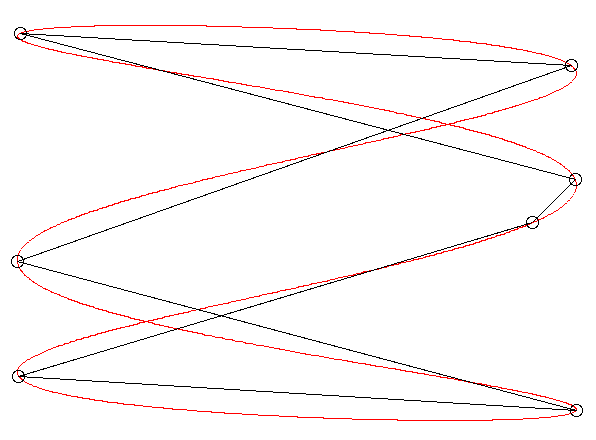
\includegraphics[width=0.3\linewidth]{Figures/lissajous01.png} &
  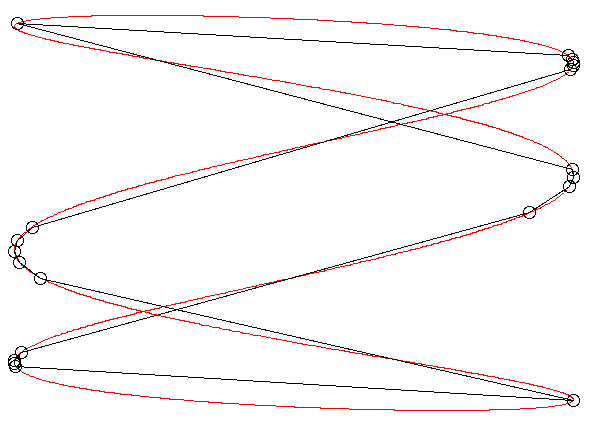
\includegraphics[width=0.3\linewidth]{Figures/lissajous001.png} &
  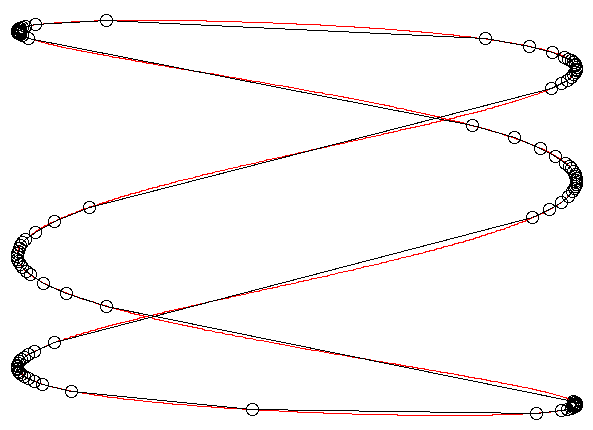
\includegraphics[width=0.3\linewidth]{Figures/lissajous0001.png}
  \end{tabular}
  \caption{\label{fig:lissajous} Lissajous Curves: 10\% deficit (left), 
1\% deficit (middle), 0.1\% deficit (right);\newline $x(t) = a * \sin(n*t 
+ c)$, $y(t) = b* \sin(t)$, $a=b=c=1$, $n=3$, $0 < t < 2\pi$}
\end{figure}

For the Lissajous curve, the optimization can be seen to be effective and 
efficient with regards to only generating vertices where the curvature is high and not wasting vertices on the relatively ``straight'' portions of the curve. In addition, the self-intersection present on this curve did not impede the generation of an optimal edge grid.

\begin{figure}[h!]
  \centering
  \begin{tabular}{ccc}
  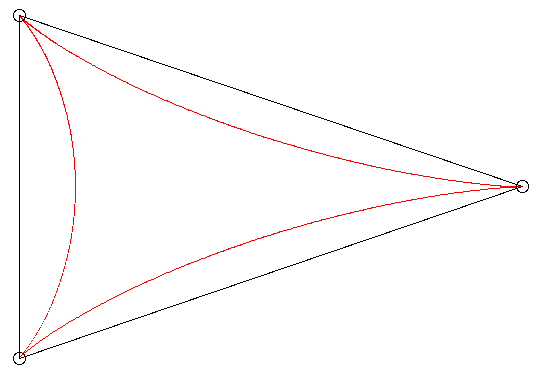
\includegraphics[width=0.3\linewidth]{Figures/tricuspoid01.png} &
  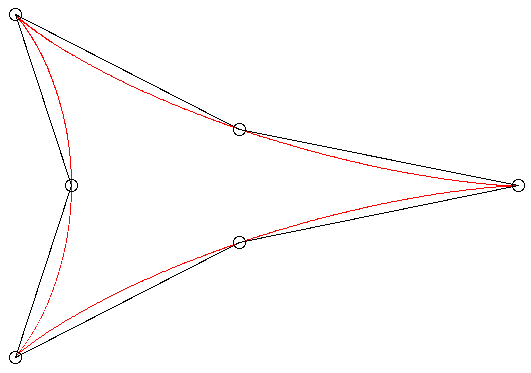
\includegraphics[width=0.3\linewidth]{Figures/tricuspoid001.png} &
  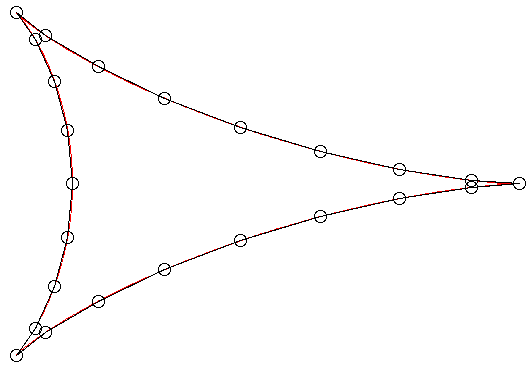
\includegraphics[width=0.3\linewidth]{Figures/tricuspoid0001.png}
  \end{tabular}
  \caption{\label{fig:tricuspoid} Tricuspoid Curve: 10\% deficit (left), 
1\% deficit (middle), 0.1\% deficit (right);\newline $x(t) = a*(2*\cos(t) 
+ \cos(2*t))$, $y(t) = a*(2*\sin(t) - \sin(2t))$, $a=1$, $0<t<2*\pi$}
\end{figure}

For the Tricuspoid curve, the algorithm for optimal point placement can be seen to be accurate with regards to placing a vertex at the discontinuities. Placing a vertex at the discontinuity is efficient since no further nodes are required to capture that feature of the curve. It can be seen that further refinements are placed elsewhere in order to capture curvature.

\begin{figure}[h!]
  \centering
  \begin{tabular}{ccc}
  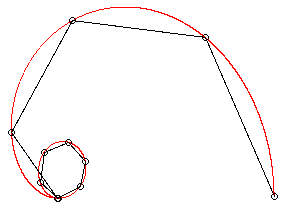
\includegraphics[width=0.3\linewidth]{Figures/cochleoid01.png} &
  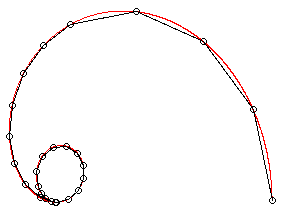
\includegraphics[width=0.3\linewidth]{Figures/cochleoid001.png} &
  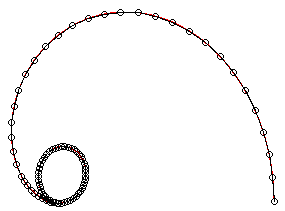
\includegraphics[width=0.3\linewidth]{Figures/cochleoid0001.png}
  \end{tabular}
  \caption{\label{fig:lastfigure} Cocheloid Curve: 10\% deficit (left), 1\% deficit (middle), 0.1\% deficit 
(right);\newline $x(t) = a * \frac{sin\left(t\right) * cos\left(t\right)}{t}, y(t) = a * \frac{sin^2\left(t\right)}{t}$, $a=1$, $0<t<2*\pi$}
  \end{figure}

For the Cochleoid curve, an interesting feature stands out: when using 
$10\%$ as the ALD, a self-intersecting discretization was generated where 
the curve does not exhibit self-intersection. This is due to the rapid 
change in curvature near the center of the spirals.  In general, this 
cannot be avoided since {\it a priori} knowledge of where the curve is 
self-intersecting would be needed to refine the discretization where 
appropriate. When refined the result is valid. The results from using $1\%$ and $0.1\%$ ALD can be seen to accurate and increase in resolution where the curve exhibits changes in curvature. On the outer portions of the spiral, the discretization is less refined than near the center of the spirals.

\Cref{tab:curvelength} and \Cref{tab:generationdata} summarize the results from discretizing the three curves. 
Each row in \Cref{tab:curvelength} shows the results from a particular percentage change in edge length that was 
used as the refinement constraint. In each row the discretization 
length of each curve is shown along with the arc-length deficit relative 
to the true length of the curve and number of segments in parenthesis. 
Each result is less than the desired arc-length deficit for the entire 
curve -- except for 1\% result for the $Lissajous$ curve which is slightly 
higher. Each row in \Cref{tab:generationdata} shows the number of segments 
corresponding to each discretization and the number of function 
evaluations. Other test results run by the authors showed similar results 
in accuracy and robustness. It should be noted that no effort was made to 
prematurely optimize the number of function evaluations, e.g., caching. 
Algorithmic optimization proved to not be needed due to the 
extremely low computational cost of the existing implementation.

\begin{table}[h!] \caption{\label{tab:curvelength} Discretization length with respect to true curve length, arc-length deficit }
\centering
\begin{tabular}{|c|c|c|c|}
\hline
 & Lissajous & Tricuspoid & Cochleoid \\
\hline
True Length & 13.0653 & 16.0 & 2.94\\
10\% deficit & 12.7123 (2.7\%) & 15.5885 (2.5\%) & 2.7916 (5.07\%)\\
1\% deficit & 12.884 (1.4\%) & 15.87 (0.78\%) & 2.916 (0.0842\%)\\
0.1\% deficit & 13.04 (0.166\%) & 15.99 (0.058\%) & 2.939 (0.076\%)\\
\hline
\end{tabular}
\end{table}

\begin{table}[h!] \caption{\label{tab:generationdata} Number of segments in final discretization, function evaluations }
\centering
\begin{tabular}{|c|c|c|c|}
\hline
 & Lissajous & Tricuspoid & Cochleoid \\
\hline
10\% deficit & 8, 1599 & 4, 615 & 11, 2337 \\
1\% deficit & 21, 4797 & 7, 1353 & 27, 6273 \\ 
0.1\% deficit & 121, 29397 & 25, 5781 & 86, 20787 \\ 
\hline
\end{tabular}
\end{table}
